\section{Method}
\label{sec:method}


% This section details our proposed autoregressive framework for multimodal conditional image generation, its core components, two-stage training paradigm, and the data construction pipeline. 
This section details an efficient autoregressive framework for controllable multimodal image generation, achieving precise image control and balancing guidance across multiple modalities with minimal cost.
\Cref{sec:Preliminary} describes the autoregressive training objective for our framework. Next, \Cref{sec:model} presents a straightforward yet efficient model architecture, detailing how the framework accommodates multimodal inputs and supports autoregressive generation.
Crucially, \Cref{sec:traing_stages} introduces a two-stage training paradigm aimed at balancing the influences of different modalities during image generation.
Finally, \Cref{sec:data_construct} describes our automated pipeline for scalable multimodal data curation.

\subsection{Preliminary}
\label{sec:Preliminary}
\textbf{Training Objective}
Our model employs \emph{teacher forcing} to predict image tokens, conditioned on (i) previously generated tokens and (ii) multimodal context $\mathbf{h}$. 
Given the multimodal condition: $\mathbf{c}^{(0)} = \{\mathcal{I}, \mathcal{T}\}$ (visual and textual inputs),
a multimodal encoder~\(\phi\) first encodes $\mathbf{c}^{(0)}$ and subsequently uses an MLP layer to project them into space of the image decoder to form a unified representation $\mathbf{h}$:
\begin{equation}
    \mathbf{H} = \text{MLP}(\phi\bigl(\mathbf{c}^{(0)}\bigr))
    = (\mathbf{h}_1, \dots, \mathbf{h}_{M}) \in \mathbb{R}^{M\times d}, \qquad \mathbf{h}_j \in \mathbb{R}^{d}.
    \label{eq:enc}
\end{equation}
where $M$ is the number of conditioning tokens, and $d$ is the dimension of the latent embeddings.
% The autoregressive decoder $\theta$, conditioned on $\mathbf{h}$, generates an image token sequence $\mathbf{y} = (y_1, \dots, y_{L})$ of length $L$. Its conditional distribution factorizes as:
Then, the AR decoder $\theta$, conditioned on $\mathbf{h}$, generates image sequence $\mathbf{y} = (y_1, \dots, y_L)$ as follows:
\begin{equation}
    \small
    \theta(\mathbf{y} \mid \mathbf{H}) = \prod_{i=1}^{L} \theta\bigl(y_i \mid y_{<i}, \mathbf{H}\bigr).
    \label{eq:factor}
\end{equation}
% where $y_{<i} = (y_1, \dots, y_{i-1})$ are the preceding tokens.
The training objective is to minimize the token-level cross-entropy loss by \emph{teacher forcing} on data $\mathcal{D}$:
\begin{equation}
\small
    \mathcal{L}_{\text{CE}}(\theta, \phi)
    = -\mathbb{E}_{(\mathbf{y}, \mathbf{c}^{(0)}) \sim \mathcal{D}}
    \left[
        \sum_{i=1}^{L}
        \log \theta\bigl(y_i \mid y_{<i}, \mathbf{H} \bigr)
    \right].
    \label{eq:ce}
\end{equation}
% Our model is trained using \emph{teacher forcing} to predict image tokens, conditioned on (i) previously generated tokens and (ii) multimodal context provided by multimodal encoder.

% Formally, given the initial multimodal condition: $\mathbf{c}^{(0)} = \{\mathcal{I}, \mathcal{T}\}$, where $\mathcal{I}$ and $\mathcal{T}$ represent visual and textual inputs, respectively. To transform the multimodal inputs $\mathbf{c}^{(0)}$ into a unified representation $\mathbf{h}$, the multimodal encoder~\(\phi\) first encodes the input into conditioning hidden states and subsequently projects them into the latent embedding space of the decoder via a MLP projection layer:

% \begin{equation}
%    \mathbf{h} = \text{MLP}(\phi\bigl(\mathbf{c}^{(0)}\bigr))
%    = (h_1, \dots, h_{M}), \qquad h_j \in \mathbb{R}^{d},
%    \label{eq:enc}
% \end{equation}
% where $M$ is the number of conditioning tokens, and $d$ is the dimensionality of the latent embeddings. 

% The autoregressive decoder $\theta$ receives the sequence $\mathbf{h}$ as a prefix and generates an output sequence of image tokens $\mathbf{y} = (y_1, \dots, y_{L})$, where $L$ is the length of the target image-token sequence. The conditional distribution modeled by the decoder factorizes autoregressively as:
% \begin{equation}
%    \theta(\mathbf{y} \mid \mathbf{h})
%    = \prod_{i=1}^{L}
%    \theta\bigl(y_i \mid y_{<i}, \mathbf{h}\bigr),
%    \label{eq:factor}
% \end{equation}
% where $y_{<i} = (y_1, \dots, y_{i-1})$ denotes the previously generated tokens.

% Training is performed using \emph{teacher forcing}, where ground-truth prefix tokens are provided at each step. The objective is to minimize the token-level cross-entropy loss over the data distribution $\mathcal{D}$:
% \begin{equation}
%    \mathcal{L}_{\text{CE}}(\theta, \phi)
%    = -\mathbb{E}_{(\mathbf{y}, \mathbf{c}^{(0)}) \sim \mathcal{D}}
%    \left[
%       \sum_{i=1}^{L}
%       \log \theta\bigl(y_i \mid y_{<i}, \phi(\mathbf{c}^{(0)})\bigr)
%    \right].
%    \label{eq:ce}
% \end{equation}
\textbf{Classifier-free Guidance} 
To enhance multimodal generation controllability, we apply Classifier-Free Guidance (CFG)~\citep{llamagen}. During training, multimodal conditioning \(\mathbf{H}\) is replaced by a learned unconditional embedding \(\mathbf{H}_u\) with probability \(p\). At inference time, token logits \(\ell_g\) are recalculated by interpolating between the conditional logits \(\ell_c\) (from \(\mathbf{H}\)) and unconditional logits \(\ell_u\) (from \(\mathbf{H}_u\)), controlled by a scaling parameter \(\lambda\):
\(\ell_g = \ell_u + (\ell_c - \ell_u) \times \lambda\).





% To enhance the multimodal conditional generation capabilities of the model, following pervious methods~\citep{llamagen}, we integrate \emph{classifier-free guidance} (CFG) during both training and inference phases. 
% Specifically, during training, we randomly replace the original multimodal inputs $c$ with learnable conditional embeddings $u$ with the possibility $p$. 
% % to encourage the model to generalize beyond strict reliance on provided conditions. 
% At inference time, the logits for each predicted token are recalculated by interpolating between the conditional logits $\ell_{c}$ obtained from original multimodal conditions $c$ and unconditional logits $\ell_{u}$ derived from the learned conditional embeddings $u$, controlled by a scaling parameter $\lambda$:
% \begin{equation}  
% \ell_{g} = \ell_{u} + (\ell_{c} - \ell_{u}) \times \lambda.
% \end{equation}  

% To enhance the controllability and guidance strength of multimodal generation, we integrate Classifier-Free Guidance (CFG) for multimodal conditional generation following pervious methods~\citep{llamagen}.
% During training, we randomly drop the multimodal conditions (e.g., replacing $\mathbf{h}$ with a learned unconditional embedding $\mathbf{h}_u$) with a certain probability $p$. 
% At inference time, the logits for the next token prediction are computed by interpolating between the conditional logits $\ell_c$ and unconditional logits $\ell_u$ using a guidance scale parameter $\lambda$:
% \begin{equation}
% \ell_{g} = \ell_{u} + (\ell_{c} - \ell_{u}) \times \lambda,
% \label{eq:cfg}
% \end{equation}
% where $\ell_c$ are derived from the model conditioned on the full multimodal input $\mathbf{h}$, $\ell_u$ are derived from the model conditioned on the learned unconditional embedding $\mathbf{h}_u$.


% Through this formulation, CFG provides flexible control over conditional strength, enabling the model to achieve a balance between coherence and diversity in the generated outputs.


\subsection{Model Design}
\label{sec:model}
As illustrated in \Cref{fig:structure}, \model architecture comprises two core components: a multimodal encoder and an autoregressive generation decoder. These components are designed to unify multimodal inputs into a shared embedding and generate image tokens sequentially conditioned on the unified embedding, respectively. 
A lightweight projection layer bridges the encoder's output to the decoder's input embedding space, enabling seamless integration between the two components.
% The multimodal encoder is responsible for unifying heterogeneous modalities (e.g., text and vision) into a shared latent space, providing conditional signals to guide the autoregressive image generator. These components are bridged via a lightweight multi-layer perceptron (MLP) projection layer, enabling seamless integration between the encoder’s output and the decoder’s input embedding space.


\textbf{Multimodal Encoder}
The multimodal encoder integrates multimodal inputs from frozen pretrained vision ($\phi_V$) and language ($\phi_L$) encoders into a shared latent space. This module projects visual features from $\phi_V$ into $\phi_L$'s embedding space using a lightweight connector module ($\psi$), yielding a unified multimodal representation $\mathbf{H} = (\mathbf{h}_1, \dots, \mathbf{h}_{M})$, where $\mathbf{h}_j \in \mathbb{R}^{d}$. 
% To address the computational demands of extensive visual tokens from $\phi_V$ while preserving detail, two architectures for $\psi$ are investigated:
Meanwhile, a critical challenge arises from the visual tokenization, where a vision encoder produces hundreds of tokens per image. It inflates the context length and leads to substantial computational costs, especially in multi-image scenarios. Compressing visual tokens can mitigate costs,  but may risk losing fine-grained visual information. To navigate this trade-off, two architectures for $\psi$ are investigated:

\begin{itemize}[left=2pt, itemsep=0.5pt,topsep=0.5pt]
    \item \textbf{MLP-based Projection}: Inspired by~\cite{liu2023llava}, we adopt a multi-layer perceptron that directly projects visual tokens to maintain detailed visual semantics with minimal information loss.
\item \textbf{Query-based Token Distillation}: We use a Query-Former~\cite{li2023blip2} to compress lengthy visual token sequences into a fixed-size representation. To guide the distillation, we condition the Query-Former on textual queries\citep{li2023blipdiffusionpretrainedsubjectrepresentation,2023instructblip} that highlight important concepts in images. It aims to guide the model to selectively extract semantically relevant visual features based on textual queries.
\end{itemize}

% The resulting multimodal encoder serves as the foundation for subsequent image generation.

% The multimodal encoder is designed to integrate vision and language inputs into a shared latent space that serves as the conditional input for the decoder. It is constructed by combining a frozen vision encoder($\phi_V$) and a frozen language model encoder ($\phi_L$), connected via a lightweight connector module ($\psi$). This connector is trained to project the features from the vision encoder into the language model's embedding space, yielding a unified multimodal representation $\mathbf{h}$.

% The multimodal encoder integrates vision ($\phi_V$) and language ($\phi_L$) inputs—both processed by frozen pretrained encoders—into a shared latent space. A lightweight connector module ($\psi$) projects visual features from $\phi_V$ into the embedding space of $\phi_L$, yielding a unified multimodal representation $\mathbf{h}$.

% To manage the computational burden of extensive visual tokens from $\phi_V$ (especially with multiple images) while retaining detail, we investigate two architectures for $\psi$:


% A critical challenge arises from the tokenization of visual inputs, where a standard vision encoder can produce hundreds of tokens per image. This inflates the context length for the decoder, especially in multi-image scenarios, leading to substantial computational costs. While visual token compression can mitigate the cost, it risks losing fine-grained visual information crucial for high-fidelity image generation. To navigate this trade-off between efficiency and information preservation, we explore two architectural designs for the connector module $\psi$:


% Through this design, the model acquires the capacity to effectively encode multimodal inputs and produce semantically coherent outputs for downstream generative decoder. Since both the decoder and the multimodal encoder operate within a shared embedding space, the model is naturally capable of producing meaningful images conditioned on the encoder's outputs. 
% As a result, this preliminary alignment phase successfully extends a text-only autoregressive image generator into one capable of handling multimodal inputs with minium cost.

% A critical challenge in this design arises from the tokenization of visual inputs. The vision encoder typically maps an image into hundreds of tokens, which significantly inflates the context length for the decoder—particularly in multi-image settings—leading to prohibitive computational overhead.
% While compressing visual tokens can alleviate this cost, it often comes at the expense of losing fine-grained visual information, which is critical for image generation.
% To navigate the trade-off between efficiency and information preservation, we explore two architectural designs for the connector module:


% \textbf{MLP-based Projection}: Following~\cite{liu2023llava}, a multi-layer perceptron directly projects visual tokens, aiming to preserve detailed visual semantics with minimal information loss.

% \textbf{Query-based Token Distillation}: Adapted from~\cite{li2023blip2}, a Query-Former compresses lengthy visual token sequences into a fixed-size representation. Textual queries guide this distillation to focus on semantically relevant visual features.

% The multimodal encoder outputs a sequence of conditioning tokens $\mathbf{h} = (h_1, \dots, h_{M})$, where $h_j \in \mathbb{R}^{d}$.


% \textbf{MLP-based Projection~\cite{liu2023llava}}. A simple multi-layer perceptron directly projects the visual tokens into the language encoder’s embedding space. This design minimizes information loss and preserves detailed visual semantics, ensuring fidelity in downstream tasks.

% \textbf{Query-based Token Distillation~\citep{li2023blip2}}. We also explore a Query-Former architecture, which compresses lengthy visual tokens sequences into a fixed-size representation. To guide this distillation process, we condition the Query-Former on textual queries that highlight semantically important concepts in input images.  It aims to guide the connector to selectively extract semantically relevant visual features by promoting interaction between visual and textual modalities.

% The resulting multimodal encoder serves as the foundation for subsequent alignment and instruction tuning stages.

% The output of the multimodal encoder, after the MLP projection layer, is a sequence of conditioning tokens $\mathbf{h} = (h_1, \dots, h_{M})$, where $h_j \in \mathbb{R}^{d}$ and $M$ is the number of conditioning tokens.
% \paragraph{Autoregressive Generation Decoder}
% The decoder is a transformer-based autoregressive generator that has the same vocabulary as the VQGAN. It is trained to synthesize images by generating image tokens autoregressively, conditioned on the multimodal encoder's outputs, and uses the VQGAN decoder to decode the generated token sequences into images. 
% Operating in a shared embedding space with the encoder's output, the decoder can naturally leverages the unified representations produced by the encoder to generate images and support the unified training via next-token prediction.

% The decoder is a transformer-based autoregressive model operating in a shared embedding space with the multimodal encoder's output. It is trained to generate images by generating a sequence of image tokens $\mathbf{y} = (y_1, \dots, y_{L})$ autoregressively, conditioned on the prefix $\mathbf{h}$ and previously generated tokens $y_{<i}$. The decoder shares the same vocabulary as the VQGAN used to encode target images into discrete tokens. The generated token sequences are subsequently decoded into images using the VQGAN decoder. This shared embedding space and autoregressive structure naturally leverage the unified multimodal representations for image generation and support unified training via next-token prediction.
\begin{figure*}[t]
\centering
\vspace{-8ex}
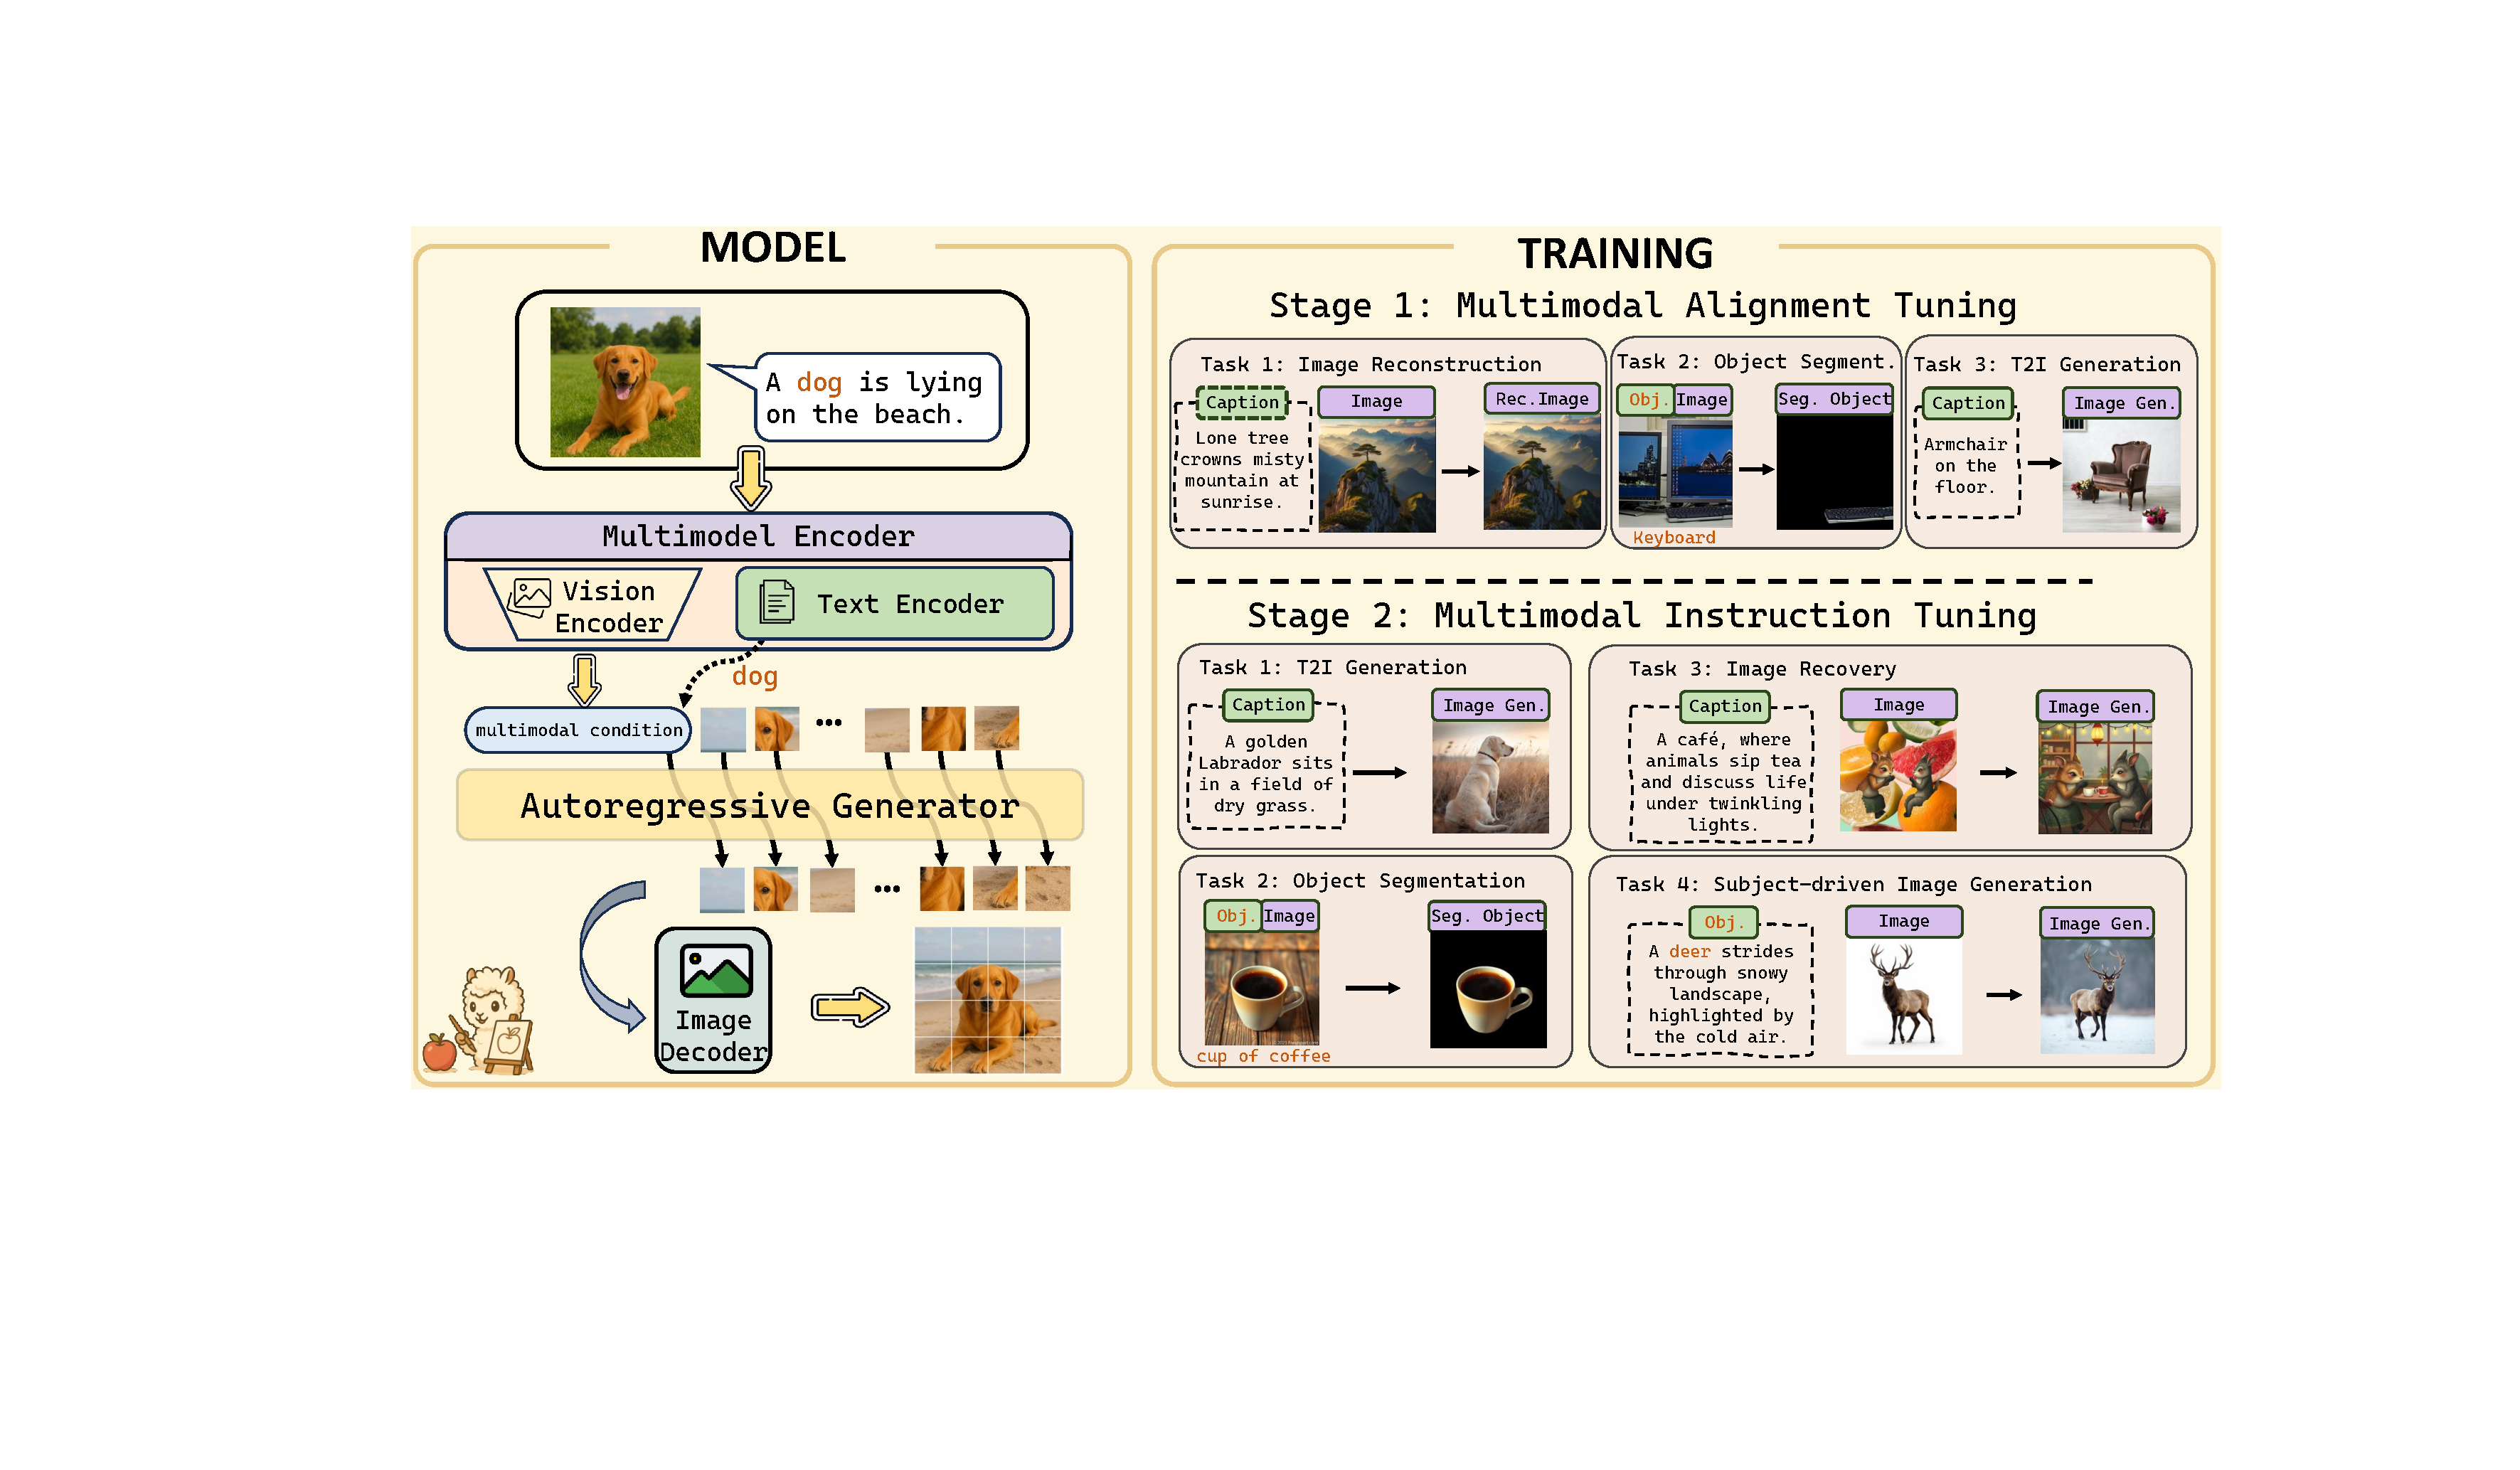
\includegraphics[width=1.0\textwidth]{figures/model_stagev2.pdf}
\caption{Overview of \model. \textbf{Left} panel illustrates the model structure, where visual and textual inputs are encoded into a unified latent to guide autoregressive image generation. \textbf{Right} panel highlights the two-stage training paradigm: (1) \textbf{Multimodal Alignment Tuning}, enabling pixel and semantic-level alignment between inputs and output tokens; and (2) \textbf{Multimodal Instruction Tuning}, compels model to effectively balance influence of different modalities.}
\label{fig:structure}
\vspace{-3ex}
\end{figure*}
\textbf{Autoregressive Generation Decoder}
A transformer-based autoregressive decoder generates a image token sequence $\mathbf{y} = (y_1, \dots, y_{L})$ conditioned on the prefix $\mathbf{H}$ generated by the multimodal encoder and previously generated tokens $y_{<i}$. It operates in a shared embedding space with the encoder's output and shares the same vocabulary as the VQGAN~\citep{Esser2020TamingTF} that is used for image tokenization.
The generated token sequences are subsequently decoded into images using the VQGAN decoder. This unified autoregressive structure facilitates unified training via next-token prediction.

% The decoder, a transformer-based autoregressive model, generates a sequence of image tokens $\mathbf{y} = (y_1, \dots, y_{L})$ conditioned on the prefix $\mathbf{h}$ and previously generated tokens $y_{<i}$. It operates in a shared embedding space with the encoder's output and uses the same discrete token vocabulary as the VQGAN employed for target image tokenization and final image synthesis from $\mathbf{y}$. This structure supports unified training via next-token prediction.

\subsection{Two-Stage Training Paradigm}
\label{sec:traing_stages}
As highlighted in the introduction, effectively aligning disparate modalities and balancing their influence are crucial challenges for multimodal conditional generation. Our carefully designed two-stage training paradigm directly addresses these issues, moving beyond initial coarse alignment to foster robust understanding and balanced integration of diverse inputs, as illustrated in \Cref{fig:structure}. 

\textbf{Stage 1: Multimodal Alignment Tuning}
While the initial connector training provides preliminary semantic alignment, we observed that the model primarily interprets visual inputs semantically like text captions, neglecting crucial visual and spatial details necessary for precise image generation. This stage is dedicated to explicitly enhancing both pixel and semantic-level modality alignment and promoting the utilization of visual information.
In Stage 1, we employ three complementary tasks:
\begin{itemize}[left=2pt, itemsep=0.5pt,topsep=0.5pt]
    \item \emph{\textbf{Image reconstruction}}, where models must faithfully reconstruct an input image conditioned on itself, with the corresponding caption randomly provided or omitted, reinforcing pixel-level fidelity.
    \item \emph{\textbf{Object segmentation}}, where models are given an input image and a target object label and must generate an end‐to‐end segmented figure for that object. This task compels the model to explicitly capture fine-grained visual details and spatial structures associated with specific semantic concepts.
    \item \emph{\textbf{T2I generation}}, using image-caption pairs to preserve and reinforce foundational generative capabilities learned during pretraining of the decoder.
\end{itemize}
Importantly, incorporating the segmentation task alongside image reconstruction mitigates the risk of the model degenerating into a trivial copy-paste behavior, such as simply replicating the input. The segmentation objective compels the model to produce semantically meaningful and spatially precise visual outputs. This complementary effect has been further analyzed and validated in \Cref{abl:stage1}.

% In Stage 1, we employ two complementary pretraining tasks:  

% \begin{itemize}[left=2pt]
% \item \emph{\textbf{image reconstruction}}, where the model must faithfully reconstruct the input image conditioned on itself, reinforcing pixel-level fidelity.
% \item \emph{\textbf{Object segmentation}}: Given an image and a target label, the model outputs an end‑to‑end segmentation of that target, cultivating fine spatial understanding and visual attention essential for visual grounding and controllable image generation.
% \item \emph{\textbf{Text-to-image generation}}: Training with image–caption pairs preserves and refines the model’s capacity to turn textual descriptions into coherent images, ensuring outputs remain firmly grounded in the input text.
% \end{itemize}

% Importantly, employing the segmentation task alongside reconstruction helps prevent from solutions—such as merely copying inputs—by requiring the model to generate semantically meaningful and spatially precise visual outputs based on multimodal conditions.

% While the preliminary alignment phase achieves coarse semantic alignment for the model, we observe that the decoder tends to treat visual inputs as text‐like captions, which predominantly captures semantic-level information, neglecting crucial pixel-level visual details necessary for precise image generation. To address this, we introduce a dedicated first stage of training designed explicitly to enhance both semantic-level and pixel-level modality alignment.

% 需要的宏包
% \usepackage{booktabs}
% \usepackage{siunitx}      % 千位分隔可选
% \sisetup{group-separator = {,}}

% %-------------------------------------------
% \begin{table}[t]
% \small
%   \begin{flushright}              % 靠右
%   \begin{minipage}{0.48\textwidth}% 右半页(≈0.5\textwidth)
%     \centering
%     \caption{Pipeline statistics}
%     \resizebox{\textwidth}{!}{%
%     \begin{tabular}{@{}l S@{}}
%       \toprule
%       \textbf{Category}       & \textbf{Value} \\
%       \midrule
%       Total                   & 3\,058\,356 \\[2pt]

%       \textbf{Stage 1}        & \textbf{2\,494\,674} \\
%       \quad t2i               & 7\,000\,000 \\
%       \quad segment           & 1\,614\,674 \\
%       \quad recover           &   180\,000 \\[2pt]

%       \textbf{Stage 2}        & \textbf{1\,313\,682} \\
%       \quad t2i               &   600\,000 \\
%       \quad segment           &   150\,000 \\
%       \quad recover           &   150\,000 \\
%       \quad subject-driven    &   413\,682 \\
%       \bottomrule
%     \end{tabular}}
%   \end{minipage}
%   \end{flushright}
% \end{table}
%-------------------------------------------


% \begin{figure*}[htbp]
%     \centering
%     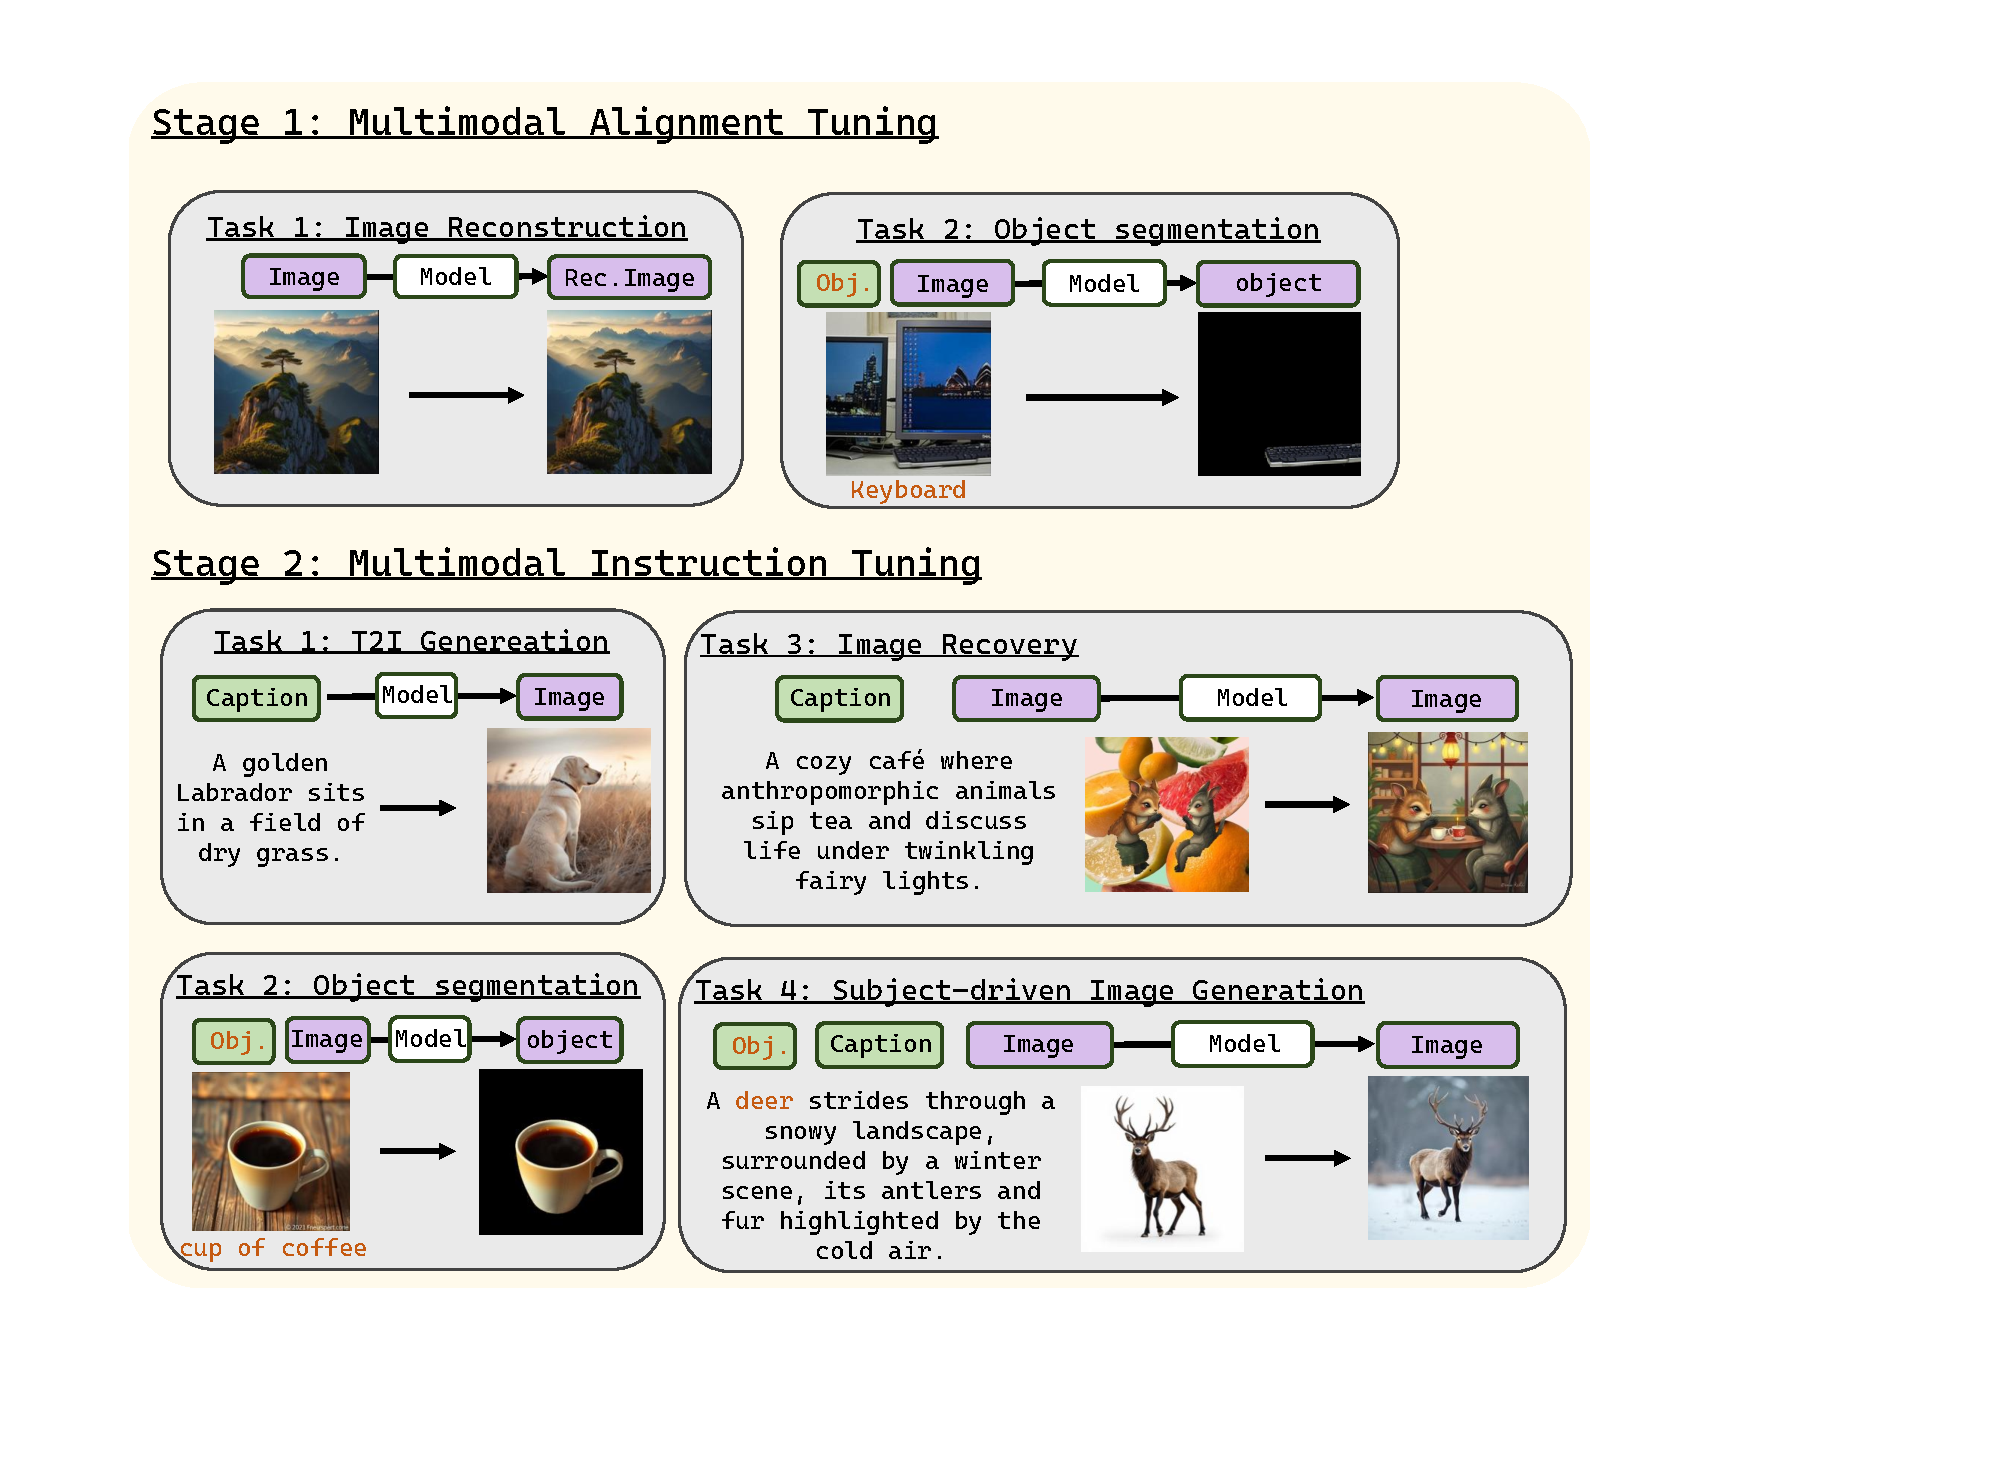
\includegraphics[width=1.0\textwidth]{figures/stages.pdf} 
%     \caption{Training Stage Placeholder
%     }
%     \label{fig:structure}
% \end{figure*}





% \begin{itemize}[left=2pt]
%     \item \emph{\textbf{Image reconstruction}}, where the model must faithfully reconstruct the input image conditioned on itself, reinforcing pixel-level fidelity.
%     \item \emph{\textbf{Object segmentation}}, where the model is given an input image and a target object label and must generate an end‐to‐end segmented figure for that object. This task compels the model to explicitly capture fine-grained visual details and spatial structures associated with specific semantic concepts.
%     \item \emph{\textbf{Text-to-image generation}}, using image-caption pairs to preserve and reinforce foundational generative capabilities learned during pretraining of the decoder.
% \end{itemize}
% Importantly, employing the segmentation task alongside reconstruction helps prevent trivial solutions—such as merely copying inputs—by requiring the model to generate semantically meaningful and spatially precise visual outputs based on the provided conditions.
% e visual outputs based on the provided conditions.


% \item \emph{\textbf{text-to-image generation}} training using image-caption pairs to preserve and reinforce foundational generative capabilities learned during pretraining of the decoder.
% \item \emph{\textbf{object segmentation}}, where the model is given an input image and a target object label and must generate an end‐to‐end segmented figure for that object. It further compels the model to explicitly capture fine-grained visual details and spatial structures associated with specific semantic concepts.
% (i)  \emph{image reconstruction}, where the model must faithfully reconstruct the input image conditioned on itself, reinforcing pixel-level fidelity; and (ii) \emph{object segmentation}, where the model is given an input image and a target object label and must generate an end‐to‐end segmented figure for that object. It further compels the model to explicitly capture fine-grained visual details and spatial structures associated with specific semantic concepts.
% Additionally, we integrate standard text-to-image generation training using image-caption pairs to preserve and reinforce foundational generative capabilities learned during pretraining of the decoder.
% Importantly, employing the segmentation task alongside reconstruction helps prevent from solutions—such as merely copying inputs—by requiring the model to generate semantically meaningful and spatially precise visual outputs based on multimodal conditions.

% Importantly, employing the segmentation task alongside reconstruction helps prevents shortcut solutions—such as directly copying inputs—by compelling the model to focus on semantically meaningful yet spatially precise visual information. Additionally, we integrate standard text-to-image generation training using image-caption pairs to preserve and reinforce foundational generative capabilities.







% The second stage of training is designed to address a central challenge in multimodal generation: ensuring the model can jointly attend to and integrate diverse input modalities in a balanced and controllable manner. 
% While the first stage focuses on aligning modalities and reinforcing the visual fidelity, Stage 2 aims to endow the model with the instruction-following ability and cross-modal reasoning capacity necessary for robust and nuanced image generation.
% Beside object segmentation and text-to-image generation, we use two additional tasks.
% To this end we adopt the multimodal instruction tuning with carefully–chosen training task. Training samples are drawn from a mixture of four complementary tasks, each targeting a distinct aspect of multimodal image generation:
% This is achieved through instruction tuning with diverse tasks designed to encourage comprehensive multimodal proficiency:

% The second stage targets enhancing the model’s capacity to jointly leverage multimodal conditions effectively during image generation, emphasizing balanced integration across modalities. 
% Specifically, we design this stage around four core training tasks to ensure comprehensive multimodal proficiency:
% \begin{itemize}[left=2pt]
% \item \emph{\textbf{Image recovery}}: Synthetically augmenting data by rotating, resizing, and compositing segmented object masks onto random backgrounds paired with original captions. This process requires the model to reconstruct the full original image, compelling it to effectively extract and integrate essential visual details from distorted contexts while relying on textual instructions to infer and restore missing components. It compels the model to fuse noisy or incomplete visual cues with textual guidance, promoting robust multimodal inference and error correction.
% \item \emph{\textbf{Subject-driven image generation}}: Conditioning on both reference images and textual instructions to serve as a final end-to-end task, fully exercising cross-modal fusion.
% \end{itemize}

% This balanced, multi-task instruction tuning ensures that the model learns to implicitly attend to and integrate both visual and textual signals harmoniously, preventing over-reliance on any single modality and yielding precise, controllable multimodal conditional generation.

\textbf{Stage 2: Multimodal Instruction Tuning}
Stage 2 aims to endow the model with robust instruction-following and cross-modal reasoning capabilities for nuanced and controllable multimodal generation, building upon the alignment and visual fidelity established in Stage 1. The model is expected to jointly attend to and integrate diverse input modalities in a balanced and controllable manner.
To achieve this, we employ a multimodal instruction tuning strategy based on a carefully curated mixture of training tasks. Specifically, we reuse the \emph{\textbf{T2I generation}} and \emph{\textbf{object segmentation}} tasks from Stage 1, maintaining identical data and formulations. These tasks respectively reinforce the model’s ability to adhere to and utilize textual and visual modalities, helping preserve foundational skills and stabilize the training process.
In addition, we introduce two novel tasks specifically designed to enhance instruction adherence and foster a balanced integration of multimodal inputs, preventing the model from over-emphasizing a single modality while neglecting others:
\begin{itemize}[left=2pt, itemsep=0.5pt,topsep=0.5pt]
    \item \emph{\textbf{Image recovery}}, where we synthetically distort images by rotating, resizing, and compositing segmented objects onto random backgrounds, then pair synthetic images with their original captions to create inputs. The model is then required to reconstruct the original image from the distorted input and corresponding caption. 
    It compels the model to extract and integrate essential visual details from noisy or incomplete visual inputs while leveraging textual cues to infer and restore missing components, promoting robust multimodal reasoning and error-correction performance.
    \item \emph{\textbf{Subject-driven image generation}}, where the model is conditioned on reference image, subject label and textual instruction to generate images. 
    It require the model to actively preserve the subject’s visual identity from the reference image while strictly adhering to the textual instructions for image generation. This task serves as a comprehensive end-to-end objective, fully exercising model’s cross-modal fusion and instruction-following abilities.
\end{itemize}
Overall, this training strategy—combining continued refinement of core capabilities with targeted instruction-based tasks—ensures the model to learn to integrate visual and textual information in a harmonious and controllable way. It mitigates over-reliance on certain modality and enables precise, controllable multimodal conditional generation, which are further discussed in \Cref{abl:stage2}. 

% \begin{figure*}[htbp]
%     \centering
%     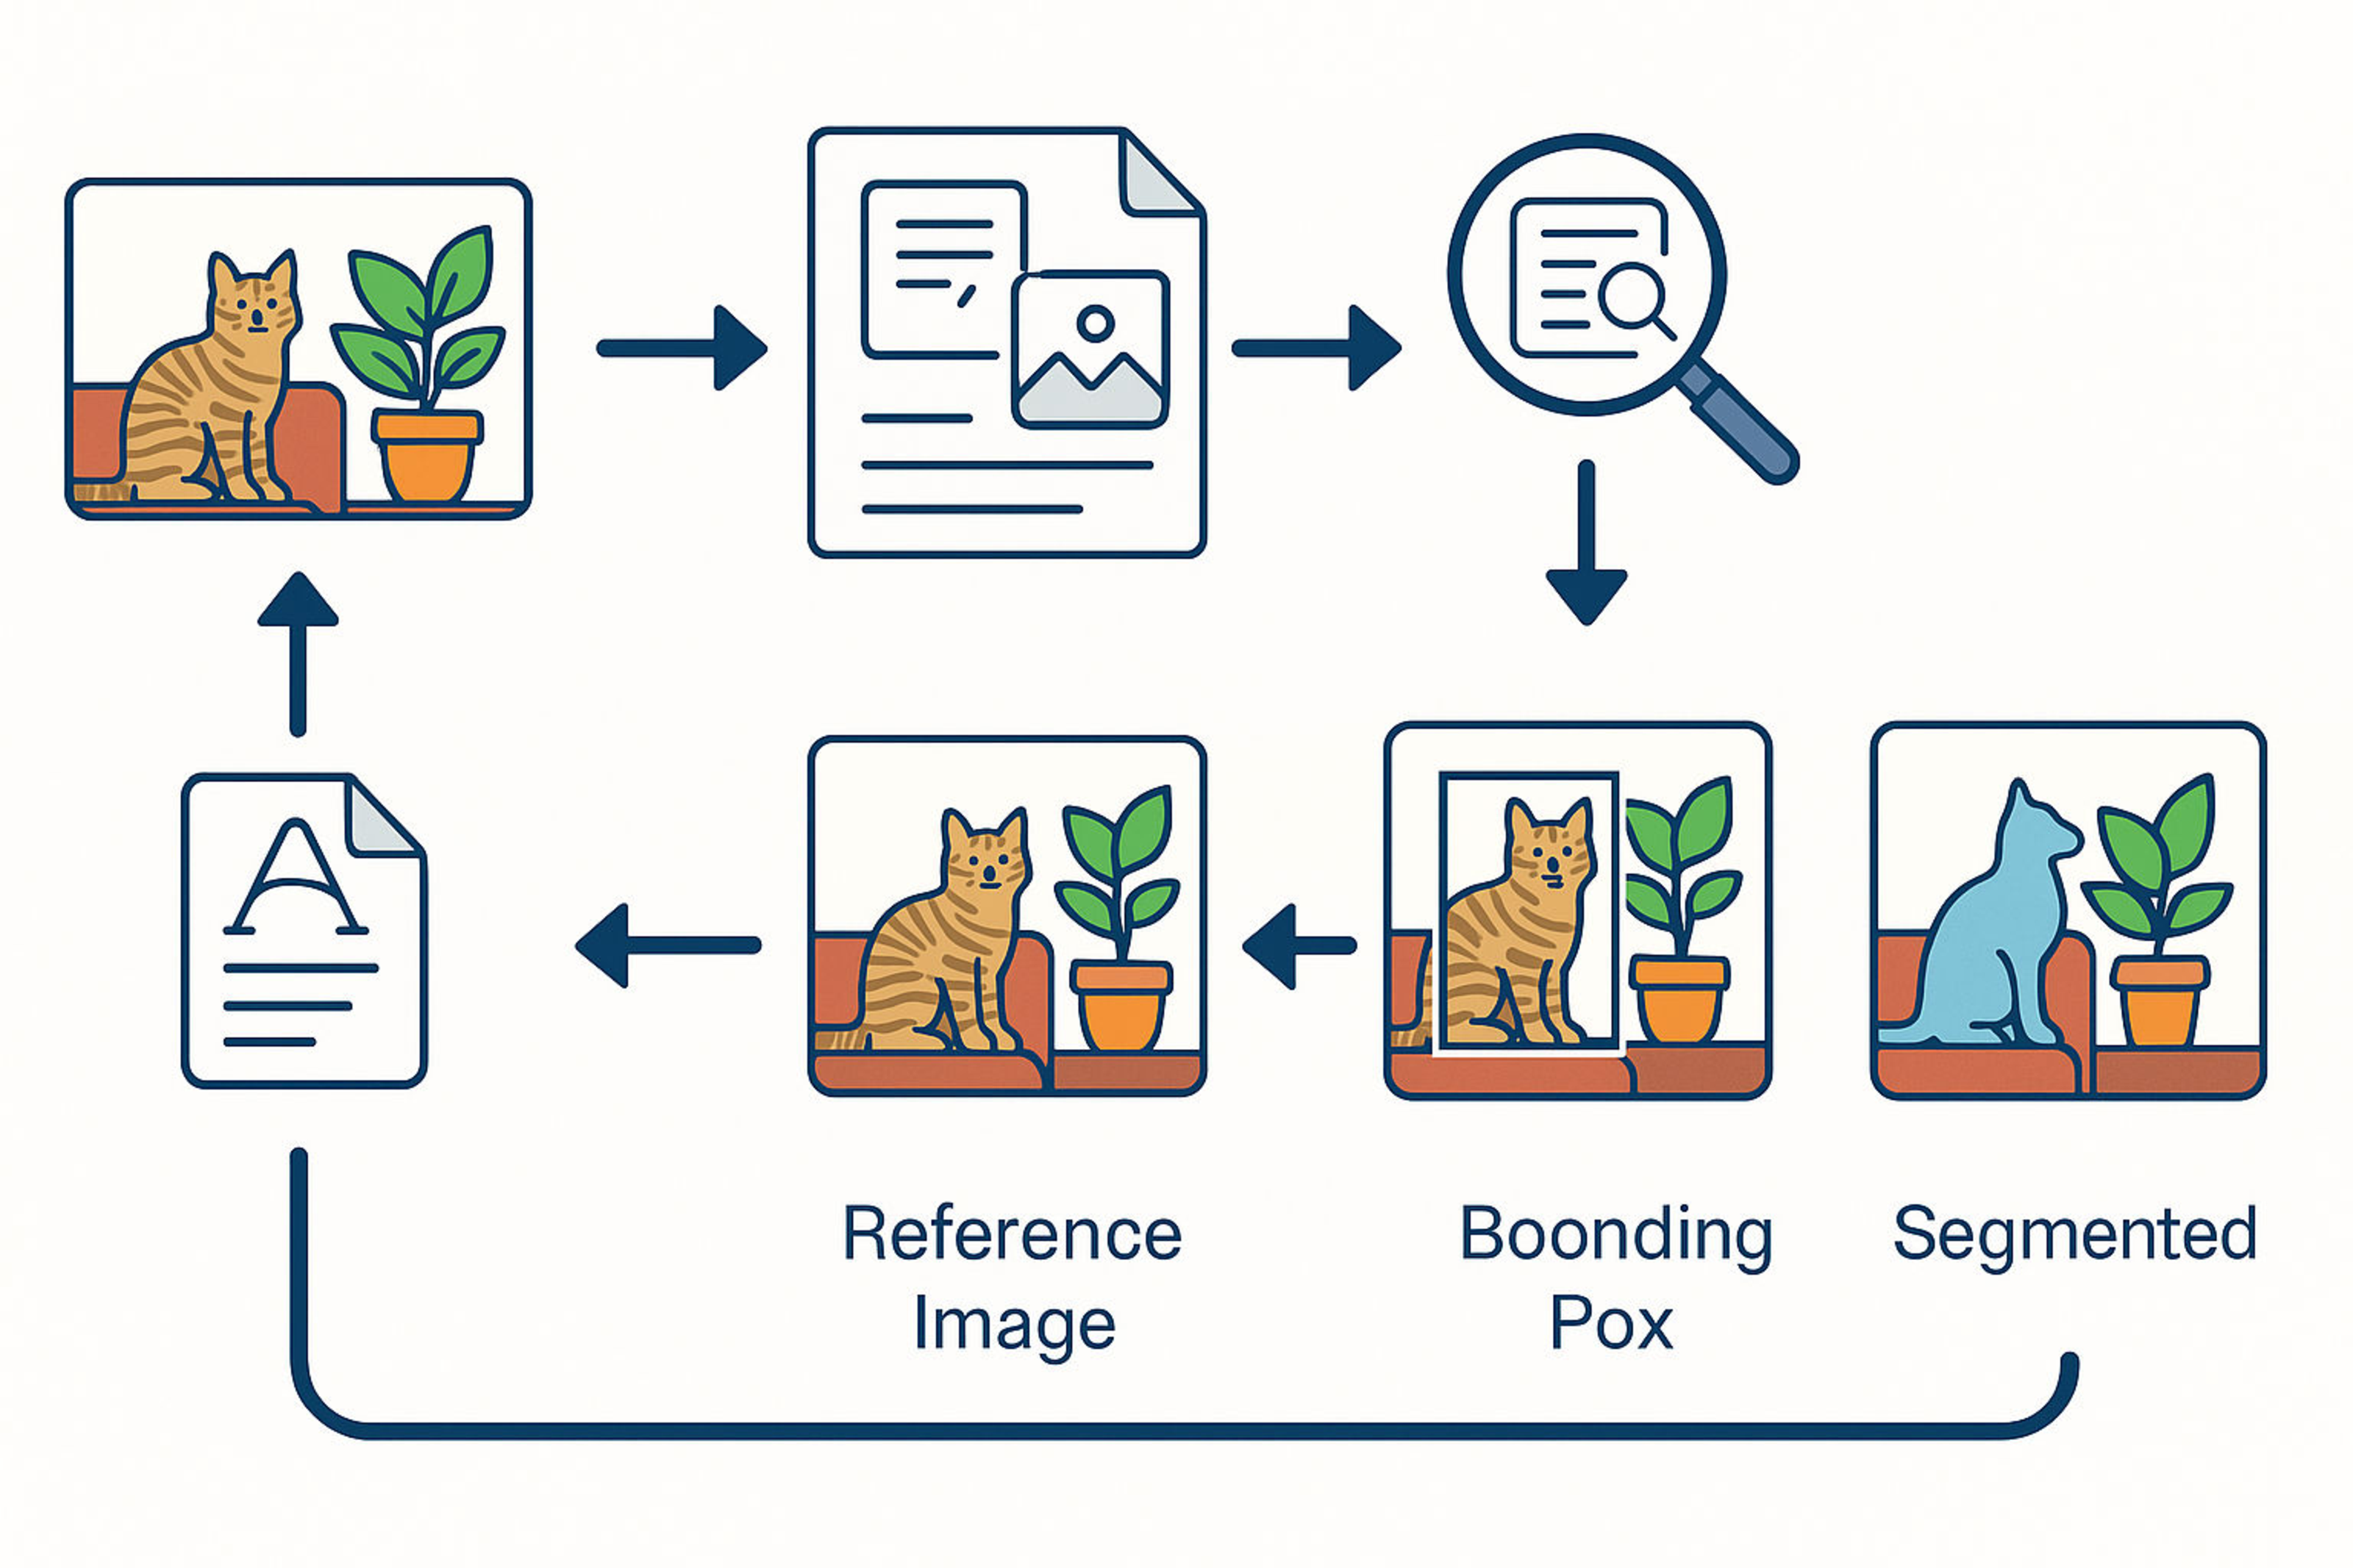
\includegraphics[width=0.8\textwidth]{figures/segment.pdf} 
%     \caption{Data construction pipeline Placeholder
%     }
%     \label{fig:structure}
% \end{figure*}


\subsection{Data Construction}
\label{sec:data_construct}

To support our two-stage training paradigm, we construct a large-scale multimodal dataset comprising approximately \textbf{3 million samples} across all training tasks. It integrates open-source resources, synthetic data, and automated annotations to ensure scalability, diversity, and strong task alignment.
For \textbf{image reconstruction} and \textbf{T2I generation}, we collect image-text pairs from datasets like CC12M~\citep{changpinyo2021cc12m} and Midjourney-Niji~\citep{midjourney-niji-1m-llavanext}.  To broaden domain coverage (e.g., human subjects, artistic scenes), we generate additional samples using T2I models like Flux.1~\citep{flux} and Stable Diffusion v3.5~\citep{2024SD3}, with prompts generated by advanced LLMs~\citep{gpt4o} to enhance semantic and visual diversity.
For \textbf{segmentation} and \textbf{image recovery}, which require fine-grained object-level annotations, we design an automated pipeline that combines state-of-the-art LMMs~\citep{Qwen2vl} with segmentation models\citep{sam}. Given an image, LMMs are queried to produce a comprehensive caption and extract a list of concrete, segmentable objects. For each object, LMMs predicts its spatial location, providing a bounding box and a set of 2D keypoints, which guide the segmentation model in producing high-quality, semantically consistent masks.
For \textbf{subject-driven image generation}, we leverage the OminiControl dataset~\citep{OminiControl}, re-captioned using LMMs to accurately extract subject-relevant descriptions. Additionally, we reverse image pairs to effectively double the usable data.
% The resulting dataset supports a wide range of multimodal tasks, including image reconstruction, T2I generation, object segmentation, and image recovery.
Data construction and formation are detailed in \Cref{sec:data_const}.




% To enable large-scale training, we design an automated pipeline that generates high-quality multimodal training data by combining open-source image datasets with the state-of-the-art vision–language models (VLMs) and segmentation models. This pipeline allows us to construct richly annotated image–text pairs containing multiple segmented foreground objects, without requiring manual labeling.

% The pipeline begins by querying a VLM to generate detailed captions and extract concrete object categories based on the image and generated caption. For each input image, we prompt the model to (1) generate a comprehensive caption that describes all visible, prominent, and foreground elements, and (2) extract a list of distinct, segmentable object names that are tangible and visually present in the image. This step ensures that only concrete and semantically meaningful visual elements are retained for downstream segmentation.

% Given the extracted object list, we then prompt the VLM again—once per object—to identify its spatial location within the image. Specifically, the model is asked to return both a tight bounding box and several representative 2D keypoints for each object. These spatial cues serve two critical roles: they constrain the region of interest for segmentation, and they reduce the likelihood of including irrelevant or overlapping background content. 

% Finally, we employ a high-performance segmentation model to extract object masks from the image, using the generated bounding boxes and keypoints. It eventually produces high-quality masks that are both semantically aligned and spatially accurate.

% By applying this pipeline to a large corpus of open-source images, we construct a multimodal dataset comprising captioned images annotated with multiple precisely segmented objects, which forms a key component of our training setup.


